\documentclass[../main.tex]{subfiles}

\begin{document}

\newcommand{\SECTIONC}{Cadenas de Markov}
\section{\SECTIONC}
\subsection{Gambler's Ruin}

\begin{frame}
  \frametitle{\SECTIONC}
  \framesubtitle{Una apuesta}

  Supongamos que tienen \$100 y les ofrezco una apuesta donde vamos a tirar una moneda 100 veces seguidas. Cada vez que salga cara su riqueza sube un 50\%, y cada vez que salga cruz su riqueza decrementa un 40\%. ¿La tomarían?
\end{frame}

\begin{frame}
  \frametitle{\SECTIONC}
  \framesubtitle{Una apuesta... Buena}

  En un principio podemos calcular la ganancia esperada: Para la primera tirada tenemos un 50\% chances de ganar \$50, y un 50\% chances de perder \$40. Por lo que esperaríamos ganar:
  \begin{gather*}
    \$50 \cdot 50\% + \$(-40) \cdot 50\% = \$5 = \$100 \cdot \%5
  \end{gather*}
  \pause El valor de la apuesta va a cambiar en las tiradas futuras, pero en todas vamos a tener una ganancia esperada del 5\%. Por lo que en promedio esperaríamos ganar un 5\% por tirada.
\end{frame}

\begin{frame}
  \frametitle{\SECTIONC}
  \framesubtitle{Una apuesta... Buena}

  Simulando esta apuesta para 10000 personas podemos ver que este promedio se cumple.

  \begin{figure}[H]
    \centering
    \includegraphics[scale=0.5]{img/mean.pdf}
  \end{figure}
\end{frame}

\begin{frame}
  \frametitle{\SECTIONC}
  \framesubtitle{Una apuesta... Buena?}

  Pero mirándolo desde otra perspectiva, si revisamos la trayectoria de 20 de estas personas, notamos que aunque a un par les va bien la mayoría no alcanza tanta riqueza.

  \begin{figure}[H]
    \centering
    \includegraphics[scale=0.5]{img/paths.pdf}
  \end{figure}
\end{frame}

\begin{frame}
  \frametitle{\SECTIONC}
  \framesubtitle{Una apuesta... Mala}

  De hecho, si lo miramos en escala logarítmica, se resalta que la mediana perdió casi todo su riqueza.

  \begin{figure}[H]
    \centering
    \includegraphics[scale=0.5]{img/logPaths.pdf}
  \end{figure}
\end{frame}

\begin{frame}
  \frametitle{\SECTIONC}
  \framesubtitle{Gambler's Ruin y ergodicidad}

  A este problema se lo conoce como la Gambler's Ruin (Ruina del Apostador). Y es un ejemplo de un sistema no-ergódico. \pause \\
  Un sistema ergódico es un sistema donde el promedio individual sobre el tiempo converge al promedio grupal. \pause La mayoría de los sistemas reales son no-ergódicos. \pause \\
  Ver un problema así nos resalta que la probabilidad no es tan directa como la solemos pensar. No es suficiente con quedarse con el cálculo de la ganancia promedio.
\end{frame}

\begin{frame}
  \frametitle{\SECTIONC}
  \framesubtitle{Ahora sí: Markov}

  Problemas como el anterior se pueden representar con lo que se conoce como un modelo de Markov. Donde tenemos un estado que cambia aleatoriamente en base al estado anterior. \pause \\
  El caso anterior es complicado de representar, por lo que vamos a ver a otro sistema más fácil de representar.

\end{frame}

\subsection{Modelando con Markov}
\newcommand{\EJC}{Un robot a través del espejo}

\begin{frame}
  \frametitle{\SECTIONC}
  \framesubtitle{\EJC}

  Vamos a modelar a un robot que se mueve sobre un tablero como el del ajedrez. \pause En específico va a empezar en la posición \(\langle 0, 0 \rangle\) en un tablero de \(3 \times 3\). En cada paso elije al azar a dónde se mueve entre los casilleros que tenga al lado. Se busca saber la probabilidad de que esté en algún casillero específico después de \(k\) pasos.

  \begin{figure}[H]
    \centering
    \chess{a1}
  \end{figure}
\end{frame}

\begin{frame}
  \frametitle{\SECTIONC}
  \framesubtitle{\EJC: Paso cero}

  \begin{figure}[H]
    \centering
    \scalebox{0.8}{
      \begin{tikzpicture}
        \CVertex{a1}{0}{0}{0}
      \end{tikzpicture}
    }
  \end{figure}
\end{frame}

\begin{frame}
  \frametitle{\SECTIONC}
  \framesubtitle{\EJC: Paso uno}

  \begin{figure}[H]
    \centering
    \scalebox{0.8}{
      \begin{tikzpicture}
        \CVertex{a1}{0}{0}{0}
          \CVertex{a2}{-3}{-3}{1}
          \CVertex{b1}{3}{-3}{2}

        \GEdge{$\frac{1}{2}$}{0}{1}
        \GEdge{$\frac{1}{2}$}{0}{2}
      \end{tikzpicture}
    }
  \end{figure}
\end{frame}

\begin{frame}
  \frametitle{\SECTIONC}
  \framesubtitle{\EJC: Paso dos}

  \begin{figure}[H]
    \centering
    \scalebox{0.8}{
      \begin{tikzpicture}
        \CVertex{a1}{0}{0}{0}
          \CVertex{a2}{-3}{-3}{1}
            \CVertex{a3}{-6}{-6}{3}
            \CVertex{b2}{0}{-6}{4}
          \CVertex{b1}{3}{-3}{2}
            \CVertex{c1}{6}{-6}{5}

        \GEdge{$\frac{1}{3}$}{1}{0}
        \GEdge{$\frac{1}{3}$}{1}{3}
        \GEdge{$\frac{1}{3}$}{1}{4}

        \GEdge{$\frac{1}{3}$}{2}{0}
        \GEdge{$\frac{1}{3}$}{2}{4}
        \GEdge{$\frac{1}{3}$}{2}{5}
      \end{tikzpicture}
    }
  \end{figure}
\end{frame}

\begin{frame}
  \frametitle{\SECTIONC}
  \framesubtitle{\EJC: Paso cero}

  \begin{figure}[H]
    \centering
    \begin{tikzpicture}
      \GVertex{1}{0}{0}{0}
      \GVertex{0}{2}{0}{1}
      \GVertex{0}{4}{0}{2}

      \GVertex{0}{0}{2}{3}
      \GVertex{0}{2}{2}{4}
      \GVertex{0}{4}{2}{5}

      \GVertex{0}{0}{4}{6}
      \GVertex{0}{2}{4}{7}
      \GVertex{0}{4}{4}{8}
    \end{tikzpicture}
  \end{figure}
\end{frame}

\begin{frame}
  \frametitle{\SECTIONC}
  \framesubtitle{\EJC: Paso uno}

  \begin{figure}[H]
    \centering
    \begin{tikzpicture}
      \GVertex{0}{0}{0}{0}
      \GVertex{$\frac{1}{2}$}{2}{0}{1}
      \GVertex{0}{4}{0}{2}

      \GVertex{$\frac{1}{2}$}{0}{2}{3}
      \GVertex{0}{2}{2}{4}
      \GVertex{0}{4}{2}{5}

      \GVertex{0}{0}{4}{6}
      \GVertex{0}{2}{4}{7}
      \GVertex{0}{4}{4}{8}

      \GEdge{$\frac{1}{2}$}{0}{1}
      \GEdge{$\frac{1}{2}$}{0}{3}
    \end{tikzpicture}
  \end{figure}
\end{frame}

\begin{frame}
  \frametitle{\SECTIONC}
  \framesubtitle{\EJC: Paso dos}

  \begin{figure}[H]
    \centering
    \begin{tikzpicture}
      \GVertex{$\frac{1}{3}$}{0}{0}{0}
      \GVertex{0}{2}{0}{1}
      \GVertex{$\frac{1}{6}$}{4}{0}{2}

      \GVertex{0}{0}{2}{3}
      \GVertex{$\frac{1}{3}$}{2}{2}{4}
      \GVertex{0}{4}{2}{5}

      \GVertex{$\frac{1}{6}$}{0}{4}{6}
      \GVertex{0}{2}{4}{7}
      \GVertex{0}{4}{4}{8}

      \GEdge{$\frac{1}{3}$}{1}{0}
      \GEdge{$\frac{1}{3}$}{1}{2}
      \GEdge{$\frac{1}{3}$}{1}{4}

      \GEdge{$\frac{1}{3}$}{3}{0}
      \GEdge{$\frac{1}{3}$}{3}{4}
      \GEdge{$\frac{1}{3}$}{3}{6}
    \end{tikzpicture}
  \end{figure}
\end{frame}

\begin{frame}
  \frametitle{\SECTIONC}
  \framesubtitle{\EJC: Full}

  \begin{figure}[H]
    \centering
    \begin{tikzpicture}
      \TVertex{0}{0}{0}{0}{0}
      \TVertex{1}{0}{2}{0}{1}
      \TVertex{2}{0}{4}{0}{2}

      \TVertex{0}{1}{0}{2}{3}
      \TVertex{1}{1}{2}{2}{4}
      \TVertex{2}{1}{4}{2}{5}

      \TVertex{0}{2}{0}{4}{6}
      \TVertex{1}{2}{2}{4}{7}
      \TVertex{2}{2}{4}{4}{8}

      \GBEdge{$\frac{1}{2}$}{0}{1}
      \GBEdge{$\frac{1}{2}$}{0}{3}

      \GBEdge{$\frac{1}{3}$}{1}{0}
      \GBEdge{$\frac{1}{3}$}{1}{2}
      \GBEdge{$\frac{1}{3}$}{1}{4}

      \GBEdge{$\frac{1}{2}$}{2}{1}
      \GBEdge{$\frac{1}{2}$}{2}{5}

      \GBEdge{$\frac{1}{3}$}{3}{0}
      \GBEdge{$\frac{1}{3}$}{3}{4}
      \GBEdge{$\frac{1}{3}$}{3}{6}

      \GBEdge{$\frac{1}{4}$}{4}{1}
      \GBEdge{$\frac{1}{4}$}{4}{3}
      \GBEdge{$\frac{1}{4}$}{4}{5}
      \GBEdge{$\frac{1}{4}$}{4}{7}

      \GBEdge{$\frac{1}{3}$}{5}{2}
      \GBEdge{$\frac{1}{3}$}{5}{4}
      \GBEdge{$\frac{1}{3}$}{5}{8}

      \GBEdge{$\frac{1}{2}$}{6}{3}
      \GBEdge{$\frac{1}{2}$}{6}{7}

      \GBEdge{$\frac{1}{3}$}{7}{4}
      \GBEdge{$\frac{1}{3}$}{7}{6}
      \GBEdge{$\frac{1}{3}$}{7}{8}

      \GBEdge{$\frac{1}{2}$}{8}{5}
      \GBEdge{$\frac{1}{2}$}{8}{7}
    \end{tikzpicture}
  \end{figure}
\end{frame}

\begin{frame}
  \frametitle{\SECTIONC}
  \framesubtitle{\EJC: Matriz}

  \begin{gather*}
    \overbrace{\begin{pmatrix}
        0 & \frac{1}{3} & 0 & \frac{1}{3} & 0 & 0 & 0 & 0 & 0  \\
        \frac{1}{2} & 0 & \frac{1}{2} & 0 & \frac{1}{4} & 0 & 0 & 0 & 0  \\
        0 & \frac{1}{3} & 0 & 0 & 0 & \frac{1}{3} & 0 & 0 & 0  \\
        \frac{1}{2} & 0 & 0 & 0 & \frac{1}{4} & 0 & \frac{1}{2} & 0 & 0  \\
        0 & \frac{1}{3} & 0 & \frac{1}{3} & 0 & \frac{1}{3} & 0 & \frac{1}{3} & 0  \\
        0 & 0 & \frac{1}{2} & 0 & \frac{1}{4} & 0 & 0 & 0 & \frac{1}{2} \\
        0 & 0 & 0 & \frac{1}{3} & 0 & 0 & 0 & \frac{1}{3} & 0  \\
        0 & 0 & 0 & 0 & \frac{1}{4} & 0 & \frac{1}{2} & 0 & \frac{1}{2} \\
        0 & 0 & 0 & 0 & 0 & \frac{1}{3} & 0 & \frac{1}{3} & 0
    \end{pmatrix}}^{\text{Matriz de transición}}
    \overbrace{\begin{pmatrix}
      1 \\ 0 \\ 0 \\ 0 \\ 0 \\ 0 \\ 0 \\ 0 \\ 0 
    \end{pmatrix}}^{\text{Este estado (\(\langle 0, 0 \rangle\))}}
  \end{gather*}
\end{frame}

\begin{frame}
  \frametitle{\SECTIONC}
  \framesubtitle{\EJC: Matriz}

  \begin{gather*}
    \overbrace{\begin{pmatrix}
        0 & \frac{1}{3} & 0 & \frac{1}{3} & 0 & 0 & 0 & 0 & 0  \\
        \frac{1}{2} & 0 & \frac{1}{2} & 0 & \frac{1}{4} & 0 & 0 & 0 & 0  \\
        0 & \frac{1}{3} & 0 & 0 & 0 & \frac{1}{3} & 0 & 0 & 0  \\
        \frac{1}{2} & 0 & 0 & 0 & \frac{1}{4} & 0 & \frac{1}{2} & 0 & 0  \\
        0 & \frac{1}{3} & 0 & \frac{1}{3} & 0 & \frac{1}{3} & 0 & \frac{1}{3} & 0  \\
        0 & 0 & \frac{1}{2} & 0 & \frac{1}{4} & 0 & 0 & 0 & \frac{1}{2} \\
        0 & 0 & 0 & \frac{1}{3} & 0 & 0 & 0 & \frac{1}{3} & 0  \\
        0 & 0 & 0 & 0 & \frac{1}{4} & 0 & \frac{1}{2} & 0 & \frac{1}{2} \\
        0 & 0 & 0 & 0 & 0 & \frac{1}{3} & 0 & \frac{1}{3} & 0
    \end{pmatrix}}^{\text{Matriz de transición}}
    \overbrace{\begin{pmatrix}
      1 \\ 0 \\ 0 \\ 0 \\ 0 \\ 0 \\ 0 \\ 0 \\ 0 
    \end{pmatrix}}^{\text{Este estado (\(\langle 0, 0 \rangle\))}}
    =
    \overbrace{\begin{pmatrix}
      0 \\ \frac{1}{2} \\ 0 \\ \frac{1}{2} \\ 0 \\ 0 \\ 0 \\ 0 \\ 0 
    \end{pmatrix}}^{\text{Siguiente estado}}
  \end{gather*}
\end{frame}

\begin{frame}
  \frametitle{\SECTIONC}
  \framesubtitle{\EJC: Resultado}

  \begin{gather*}
    M^{k} v_{0} = \overbrace{v_{k}}^{\text{Distribución del \(k\)-ésimo estado}}
  \end{gather*} \pause
  Por lo que el resultado a lo pedido es
  \begin{gather*}
    P(\text{Esté en la posición } \langle r, c \rangle \text{ en el \(k\)-ésimo paso}) = (M^{k}v_{0})_{3r + c} = (v_{k})_{3r + c}
  \end{gather*}
\end{frame}

%TODO: Alguna conclusión o generalización?

\end{document}
